The design of OMDoc/MMT predates \pn, and we have reported on it previously~\cite{Kohlhase:OMDoc1.2,RabKoh:WSMSML13,DehKohKon:iop16,KohMuePfe:kbimss17}.
Therefore, we focus on the design of ULO here, which we report in Section~\ref{sec:ulo}.

Then, in Section~\ref{sec:isabelle}, we report on \taskref{dksbases}{isabelle}, which exports the Isabelle knowledge base into OMDoc/MMT and ULO.  The latter includes the generation of ULO data from concrete libraries in RDF format.  The resulting Isabelle Theorem dataset is massive, resulting in \ednote{insert OMDoc size} $\approx 10^7$ RDF triples, requiring many CPU-hours to generate.  In parallel work, we have developed a similar export of the Coq library ~\cite{MueRabSac:cltg19}, which we do not present in detail here.

Finally, in Section~\ref{sec:uloappl}, we demonstrate how to leverage these lightweight, high-level representations in practice.
As an example application, we set up a relational query engine based on Virtuoso.
It answers complex queries instantaneously, and even simple queries allow obtaining information that was previously impossible or expensive to extract.
Example queries include asking for all theorems of any library whose proof uses induction on $\mathbb{N}$,
%all theorems by a Michael Kohlhase or Makarius Wenzel, or 
%all theorems with incomplete Proofs,
or all authors of theorems ordered by how many of the proofs are incomplete,
%the average time it takes to check the proof assistant to check their theorems,
or all dependency paths through a particular library ordered by cumulative check time (which would enable optimized regression testing).
% \ednote{FR: make sure we mention motivating examples here that we can handle; then refer back to them when giving examples in Sect.~\ref{sec:appl}}

\subsection{The Upper Library Ontology}\label{sec:ulo}
We use a simple data representation language for upper-level information about libraries. This \textbf{Upper Library Ontology} (ULO) describes objects in theorem prover libraries, their taxonomy, and relations as well as organizational and information.
The ULO allows the export of upper-level library data from theorem prover libraries as RDF/XML files (see \S\ref{sec:isabelle}), and gives meaning to them. 
The ULO is implemented as an OWL2 ontology, and can be found at \url{https://gl.mathhub.info/ulo/ulo/blob/master/ulo.owl}.
All new concepts have URIs in the namespace \url{https://mathhub.info/ulo}, for which we use the prefix \lstinline|ulo:| below.
In the sequel we give an overview of the ULO, and we refer to \cite{ULODoc:on} for the full documentation.

\subsubsection{Individuals}

Individuals are the atomic objects relevant for mathematical libraries.
Notably, they do not live in the {\ns} namespace but in the namespace of their library.

These include in particular all globally named objects in the library such as theories/modules/etc, types, constants, functions, predicates, axioms, theorems, tactics, proof rules, packages, directories, files, sections/paragraphs, etc.
For each library, these individuals usually share a common namespace (an initial segment of their URI) and then follow a hierarchic schema, whose precise semantics depends on the library.

Additionally, the individuals include other datasets such as
researchers as given by their ORCID or real name, 
research articles as given by their DOI,
research software systems as given by their URI in swMATH\footnote{\url{https://swmath.org/software/NUMBER}}, 
or MSC\footnote{\url{http://msc2010.org/resources/MSC/2010/CLASS}} and ACM\footnote{\url{https://www.acm.org/publications/class-2012}} subject classes as given by their respective URIs.
These individuals are not generated by our export but may occur as the values of key-value attributions to the individuals in prover libraries.

\subsubsection{Classes}

Classes can be seen as unary predicates on individuals, tags, or soft types.
The semantic web conventions tend to see them simply as special individuals that occur as values of the is-a property of other individuals.
%With that convention in place, they are special cases of individuals, albeit in the {\ns} namespace.
Figure~\ref{fig:classes} gives an overview of the most important classes in the ULO.

\paragraph{Logical Role}
The logical classes describe an individual's formal role in the logic, e.g., the information that $\mathbb{N}$ is a type but $0$ an object.

\ind{theory}{\isabelle\coq} refers to any semantically meaningful group of named objects (declarations).
There is a wide range of related but subtly different concepts using words such theory, class, signature, module type, module, functor, locale, instances, structure, locale interpretation, etc.

\newcommand{\truthType}{\ind{predicate}\xspace}
\newcommand{\truthObject}{\ind{statement}\xspace}

Inside theories, we distinguish five classes of declarations depending on what kind of entity is constructed by an individual:
\ind{type}{\isabelle\coq} if it constructs types or sorts like $\mathbb{N}$ or $list$; \ind{function}{\isabelle\coq} if it constructs inhabitants of types like $+$ or $nil$; \truthType{\isabelle\coq} if it constructs booleans/propositions such as $=$ or $\mathrm{nonEmpty}$; \truthObject{\isabelle\coq}%
\footnote{We have reconsidered the name of this class many times: all suggested names can be misunderstood.
The current name stems from the intuition that axioms and theorems are the most important named truth-establishing declarations, and \emph{statement} is a common way to unify them.
Arguably more systematic would be \emph{proof}: anything that establishes truth is formalized as an operator that constructs a proof.}
if it establishes the truth of a proposition such as any axioms, theorem, inference rule; and finally \ind{universe}{\isabelle\coq} if it constructs collections of types such as $\mathrm{Set}$ or $\mathrm{Class}$.

\begin{wrapfigure}r{3.5cm}\vspace*{-2.5em}
  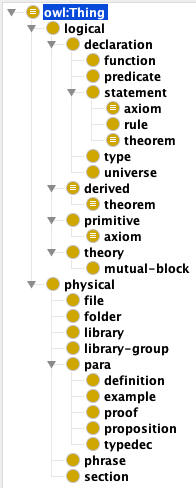
\includegraphics[width=3.5cm]{classes}\vspace*{-.5em}
  \caption{ULO Classes}\label{fig:classes}\vspace*{-3em}
\end{wrapfigure}
Note that while we hold the distinction of these five classes to be universal, concrete logics may not always distinguish them syntactically.
For example, HOL identifies functions and predicates, but the extractor can indicate whether a declaration's return type is the distinguished type of booleans.
Similarly, Curry-Howard-based systems identity predicates and types as well as statements and objects, which an extractor may choose to separate.

% The semantically meaningful sorts come in three pairs each containing a type-like sort $s$ and an object-like sort $t$.
% Intuitively, individuals $i$ and $j$ of sorts $s$ and $t$ occur together in some kind of is-a or is-instance-of relation such as a typing judgment $j:i$.


% \ind{type} and \ind{function}: These are the typical sorts of most objects.
%  In first-order logic, they correspond to sorts and function symbols.
%  In type theories, they correspond to type and function symbols.

%  FR: It's difficult to come up with good names for these. So I've introduced macros for now.
%  predicate used to be called 'proposition' but that is used elsewhere as a kind of theorem
%
%\truthType and \truthObject\ednote{these names are open for discussion, see source code}: In the Curry-Howard representation, these are special cases of \ind{type} and \ind{function}, but for relating and querying libraries, it is valuable to distinguish them, and even for systems that internally use the Curry-Howard representation, it is desirable to tease them apart.  $i$ is a \truthType if it is/returns a boolean, formula, judgment etc. (regardless of its truth value), and $i$ is a \truthObject if it is/returns anything that establishes the truth of such a formula (e.g.\ axiom, theorem, proof rule).
%
%We use the \ind{rule} class to indicate that a statement can be or is interpreted as a simplification or rewrite rule, Coq has more roles like these, e.g.: \ind{coercion} (to automatically cast a value from a type to another type), \ind{hint} (to automatically try to apply it when doing blind proof search), \ind{instance} of a type-class, to be used during user-guided proof search when guessing the parameters marked to be guessed using type-classes, \ind{morphism} to be used by setoid-rewriting tactics, etc.

Orthogonally to the above, we distinguish declarations by their definition status: \ind{primitive}{\isabelle\coq} if it introduces a new concept without a definition such as an urelement or an axiom; and \ind{derived}{\isabelle\coq} if it can be seen as an abbreviation for an existing concept like a defined operator or a theorem.
For example, intersecting the classes \truthObject and \ind{derived}, we capture all theorems.

While the primitive-derived distinction is clear-cut for definition-based systems like Coq, it is trickier for axiom-based systems like Isabelle: an Isabelle definition actually consists of a primitive concept with a defining axioms for it.
For that purpose, we introduce the \ind{defines} property in \S\ref{sec:objprops}.
%\ednote{CSC: possible alternative names: \ind{defined} and \ind{declared}. Question: is it worth distinguish between defined implicitly, e.g. as the unique object that has some property vs explicitly, by describing the object?}
  
\paragraph{Physical Role}
The physical classes describe an individual's role in the physical organization of a library.
This includes for an individual $i$:
\begin{compactitem}
 \item \ind{section}{\isabelle} if $i$ is an informal grouping inside a file (chapter, paragraph etc.)
 \item \ind{file}{\coq} if $i$ is a file
 \item \ind{folder}{\coq} if $i$ is a grouping level above source files inside a library, e.g., a folder, sub-package, namespace, or session
 \item \ind{library}{\coq} if $i$ is a library. Libraries have logical URIs and serve as the root objects containing all other individuals.
 A library is typically maintained and distributed as a whole, e.g., via a GitHub repository.
 A library has a logical URI and the URIs of individuals are typically formed relative to it.
 \item \ind{library-group}{\coq} if $i$ is a group of libraries, e.g., a GitHub group.
\end{compactitem}

\noindent In addition we define some classes for the lowest organizational level, called \emph{logical paragraphs}.
These are inspired by definition--example--theorem--proof seen in informal mathematics and often correspond to {\LaTeX} environments.
In formal libraries, the individuals of these classes may be the same as the ones for the logical classes or different ones.
For example, a document-oriented system like Isabelle could assign a physical identifier to a paragraph and a different logical one to the formal theorem inside it.
These identifiers could then have classes \ind{proposition} and \truthObject respectively. %\ednote{FR: This is a good example of our names still being unintuitive.}
A purely formal system could omit the physical class or add it to the logical identifier, e.g., to mark a logical definition as an \ind{example}{\coq} or \ind{counter-example}.
Some of these, in particular, theorems given informal classes like ``Lemma'' or ``Hauptsatz'', a string which can be specified by the \ind{paratype} relation (see below).
 
%We use the class \ind{phrase} for intra-sentential fragments of in mathematical text and formulae, these include symbols, declarations, and quantifications.

\subsubsection{Properties}\label{sec:objprops}

All properties are binary predicates whose first argument is an individual.
The second argument can be an individual (\textbf{object property}) or a value (\textbf{data property}).
Unless mentioned otherwise, we allow the same property to be used multiple times for the same individual.

The two kinds are often treated differently.
For example, for visualization as a graph, we can make individuals nodes (using different colors, shapes etc. depending on which classes a node has) and object properties edges (using different colors, shapes, etc. for different properties).
The data properties on the other hand would be collected into a key-value list and visualized at the node.
Another important difference is during querying: object properties are relations between individuals and thus admit relational algebra such as union and intersection or symmetric and transitive closure.
Data properties on the other hand are usually used with filters that select all individuals with certain value properties.

\paragraph{Library Structure}
Individuals naturally form a forest consisting e.g., of (from roots to leafs) library groups, libraries, folders, files, section, modules, groups of mutual recursive objects, constants.
Moreover, the dependency relation between individuals (in particular between the leaves of the forest) defines an orthogonal structure.

$\ind{specifies}(i,j)${\isabelle\coq} expresses that $j$ is a child of $i$ in the forest structure.
Thus, taking the transitive closure of \ind{specifies} starting with a library, yields all individuals declared in a library.

$\ind{uses}(i,j)${\isabelle\coq} expresses that $j$ was used to check $i$, where $j$ may include extra-logical individuals such as tactics, rules, notations.
A very frequent case is for $j$ to be an occurrence of a logical individual (e.g. a constant or a theorem). The case of occurrences leads to the question about what information can be attached to an occurrence. Examples could be: the number of repetitions of the occurrence; whether the occurrence of a constant induces a dependency on the type only, or on the actual definition as well; where the occurrence is located (e.g. in the statement vs proof, in the type vs body or in more specific positions, like as the head symbol of the conclusion, see~\cite{AGSTZ:ContMathSearchWhelp04} for a set of descriptions of positions that is useful for searching up to instantiation). For now we decided to avoid to specify occurrences in the ontology, for the lack of a clear understanding of what properties will really be useful for applications. Integrating the ULO ontology with occurrenes is left for future work towards ULO 1.0.

\paragraph{Semantic Relations between Declarations}
Relational representations treat individuals as black boxes.
But sometimes it is helpful to expose a little more detail about the internal structure of a declaration.
For that we define the following properties:
\begin{compactitem}
 \item $\ind{defines}(i,j)$ is used to relate a declaration $j$ to its definition $i$ if the two have different identifiers, e.g., because they occur in different places in the source file, or because $i$ is a defining axiom for a constant $j$.
 \item $\ind{justifies}(i,j)${\isabelle} relates any kind of argument $i$ to the thesis $j$ it supports. The most important example is relating a proof to its theorem statement if the two have different identifiers.
 \item $\ind{instance-of}(i,j)${\isabelle\coq} relates a structuring declaration $j$ to the theory-like entity $i$ that realizes, e.g., a module to its module type, an instance to its (type) class, a model to its theory, or an implementation to its specification.
 \item $\ind{generated-by}(i,j)$ expresses that $i$ was generated by $j$, e.g., the user may define an inductive type $j$ and the systems automatically generated an induction schema $i$.
 \item $\ind{inductive-on}(i,j)${\isabelle} expresses that $i$ is defined/proved by induction on the type $j$.
\end{compactitem}

\paragraph{Informal Cross-References}
First we define some self-explanatory cross-references that are typically (but not necessarily) used to link individuals within a library. These include \ind{same-as}, \ind{similar-to}, \ind{alternative-for}, \ind{see-also}, \ind{generalizes}, and \ind{antonym-of}.

Second we define some cross-references that are typically used to link a knowledge item in a library to the outside.
Of particular relevance are:
\begin{compactitem}
 \item $\ind{formalizes}(i,j)$ indicates that $j$ is an object in the informal realm, e.g., a theorem in an article, that is formalized/implemented by $i$.
 \item $\ind{aligned-with}(i,j)$ indicates that $i$ and $j$ formalize/implement the same mathematical concept (but possibly in different ways).
% \item \ind{inspired-by} and  are self-explanatory.
\end{compactitem}

\paragraph{Data Properties}
All properties so far were object properties.
Data properties are mostly used to attach metadata to an individual.
We do not introduce new names for the general-purpose metadata properties that have already been standardized in the Dublin Core such as
\verb|dcterms:creator|,
\verb|dcterms:title|,
\verb|dcterms:contributor|,
\verb|dcterms:description|,
\verb|dcterms:date|,
\verb|dcterms:isVersionOf|,
\verb|dcterms:source|,
\verb|dcterms:license|.
But we define some new data properties that are of particular interest for math libraries:
\begin{compactitem}
 \item $\ind{name}(i,v)${\isabelle\coq} attributes a string $v$ to a declaration that expresses the (user-provided) name as which it occurs in formulas.
 This is necessary in case an individual generated URI is very different from the name visible to users, e.g., if the URI is generated from an internal identifier or if the name uses characters that are illegal in URIs.
 \item $\ind{sourceref}(i,v)${\isabelle\coq} expresses that $v$ is the URI of the physical location (e.g., file, line, column in terms of UTF-8 or UTF-16 characters) of the source code that introduced $i$.
 \item $\ind{docref}(i,v)${\coq} expresses that $v$ is the URI reference to a place where $f$ is documented (usually in some read-only rich text format).
 \item $\ind{check-time}(i,v)${\isabelle} expresses that $v$ is the time (a natural number giving a time in milliseconds) it took to check the declaration that introduced $i$.
 \item $\ind{external-size}(i,v)${\isabelle} expresses that $v$ measures the source code of $i$ (similar to positions above).
 \item $\ind{internal-size}(i,v)${\coq} expresses that $v$ is the number of bytes in the internal representation of $i$ including inferred objects and generated proofs.
 \item $\ind{paratype}(i,v)${\isabelle} gives the ``type'' of a logical paragraph, i.e. something like ``Lemma'',  ``Conjecture'', \ldots. This is currently a string, but will become a finite enumeration eventually.
\end{compactitem}
Locations, sizes, and times may be approximate

\paragraph{Organizational Status}
Finally, we define a few (not mutually exclusive) classes that library management--related information such as being experimental or deprecated.
Many of these are known from software management in general.
The unary properties are realized as data properties, where the object is an explanatory string, the binary relations as object properties. 
An important logic-specific class is \ind{automatically-proved} --- it applies to any theorem, proof step, or similar that was discharged automatically (rather than by an interactive proof).

%%% Local Variables:
%%% mode: latex
%%% mode: visual-line
%%% fill-column: 5000
%%% TeX-master: "report"
%%% End:

%  LocalWords:  textbf organizational ednote swMATH irrelavant mathbb newcommand xspace mathrm emph formalized wrapfigure vspace includegraphics setoid-rewriting sec:objprops organization compactitem visualization visualized


\subsection{Exporting the Isabelle Knowledge Base}\label{sec:isabelle}
\subsubsection{Isabelle Overview}

Isabelle is a generic platform for tools based on formal logic.
It is generally known for its Isabelle/HOL library, which provides many theories and add-on tools (implemented in Isabelle/ML) in its \texttt{Main} theory and the \texttt{main} group of library sessions.
Some other (much smaller) Isabelle logics are FOL, LCF, ZF, CTT (an old version of Martin-L\"of Type Theory), but today most Isabelle applications are based on HOL.
The foundations of Isabelle due to Paulson~\cite{paulson700} are historically connected to \emph{logical frameworks} like Edinburgh LF: this fits nicely to the LF theory used in logic formalizations in MMT.
User contributions are centrally maintained in AFP, the \emph{Archive of Formal Proofs} (\url{https://www.isa-afp.org}).

From a high-level perspective, Isabelle is better understood as \emph{document-oriented proof assistant} or \emph{document preparation system} for domain-specific formal languages~\cite{Wenzel:IIdsflitd18}.
It allows flexible nesting of sub-languages, and types, terms, propositions, and proofs (in Isabelle/Isar) are merely a special case of that.
The result of processing Isabelle document sources consists of internal data structures in Isabelle/ML that are private to the language implementations.
Thus it is inherently difficult to observe Isabelle document content by external tools, e.g.\ to see which $\lambda$-terms occur in nested sub-languages.

Isabelle/PIDE \cite{Wenzel:2014:ITP-PIDE}, the Prover IDE framework, integrates all
activities of development for proofs and programs into a
\emph{semantic editor} Isabelle/jEdit. While the user is composing
text, the prover provides real-time feedback about its meaning: that
rich PIDE markup information can be rendered as conventional GUI
metaphors (e.g.\ text color, squiggly underline, tooltips, hyperlinks,
icons in the border) \cite{Wenzel:2019:MKM}. It is also possible to
run Isabelle/PIDE in ``headless mode'', to let some Isabelle/Scala
program observe markup as a formal library is processed in
Isabelle/ML.

The standard distribution of Isabelle\footnote{\url{https://isabelle.in.tum.de}} includes the
Isabelle/HOL library with various applications, but the main bulk of
applications is in the \emph{Archive of Formal Proofs}
(AFP)\footnote{\url{https://www.isa-afp.org}}, which is organized like
a scientific online journal. In August 2019, Isabelle/AFP had 492
articles by 331 authors, comprising 120\,MB source text total. Formal
checking requires approx.\ 50h CPU time or 2h elapsed time on high-end
multicore hardware. The result is a collection of heap images for the
internal state of Isabelle/ML and some HTML or PDF documents that
resemble conventional mathematical texts (with relatively little
formal markup being used here).


% % % % % % % % % % % % % % % % % % % % % % % % % % % % % % % % % % % % % % % % % % % % % % % % % % %
\subsubsection{General Technical Aspects of Exporting Isabelle Knowledge Bases}

Isabelle/ML is the \emph{internal implementation language} for logic-based tools, has direct access to the inference kernel in the manner of the ``LCF-approach'' \cite{Gordon-Milner-Wadsworth:1979}.
Isabelle/Scala is the \emph{external interface language} to manage Isabelle processes and
resulting content: it has access to the physical world with GUI frameworks, TCP servers, database engines etc.

To support exports like ours systematically, Wenzel had previously already instrumented the theory processing in Isabelle/ML to allow arbitrary \emph{presentation} for every theory node as it is finished: an ML function gets access to all commands with their intermediate theory
values; it can extract suitable information and \emph{export} it via a private channel to Isabelle/Scala.
The standard configuration of Isabelle provides options like \verb,export_theory, or \verb,export_proofs, to externalize certain aspects of theory content as a \emph{session database}.
For example, see command-line tools like \verb,isabelle build -o export_theory HOL-Analysis, to build such a database (for SQLite) and \verb,isabelle export -l HOL-Analysis, to query it later on.

Isabelle/Scala provides direct access to session builds and their results as an API for \emph{typed functional-object-oriented programming}: this is more robust and versatile than command-line tools.
For our export, we use the Isabelle/Scala APIs to provide dedicate command-line \verb,isabelle mmt_import,: options and arguments similar to \verb,isabelle build, specify a collection of sessions to be processed, the results are given to the MMT Scala API to write files in OMDoc format; there is extra output of RDF/XML files.

Our export (Isabelle repository version e6fa4b852bf9) turns this content into OMDoc and RDF/XML.
Our command-line tool uses regular Scala APIs of MMT (without intermediate files), and results are written to the file-system in OMDoc and RDF/XML format.
It runs a Prover IDE session (PIDE) under program control: a collection of \emph{sessions} with corresponding \emph{theories} is turned into formal source edits that are given to Isabelle/PIDE for semantic processing; the underlying prover process continuously produces markup reports as it explores the meaning of the source.
Whenever some theory node (with all imports) is finished, a separate Scala operation is invoked to \emph{commit} the result as
PIDE \emph{document snapshot}.
Thus the application can harvest theory exports produced up to that point, and the system can edit-out already processed theory-subgraphs to free resources, while the overall process is still running.

Thus the full material of AFP (hundreds of sessions, thousands of theories) can be digested on a high-end multicore machine within
approx. 24h elapsed time using 60 GB RAM for Isabelle/ML and 30 GB RAM for Isabelle/Scala.
This is approximately a factor 10 more than a conventional batch build, but the PIDE session is able to ``see'' more detailed information about the formal meaning of the sources (e.g.\ the use of term constants within the theory text, like the IDE front-end uses to provide hyperlink operations).

% % % % % % % % % % % % % % % % % % % % % % % % % % % % % % % % % % % % % % % % % % % % % % % % % % %
\subsubsection{Exporting Symbolic Knowledge in OMDoc/MMT Format}

We export all \emph{logical foundations} of theory documents (types, consts, facts, but \emph{not} proof terms), and aspects of \emph{structured specifications} (or ``little theories'') (locales and locale interpretations, which also subsumes the logical content of type classes).
Figure~\ref{fig:isabellemmt} shows a screenshot of the MMT browser showing a small part (the definition of binomial coefficients in Isabelle/HOL) of the exported Isabelle knowledge base.

\begin{figure}[ht]
  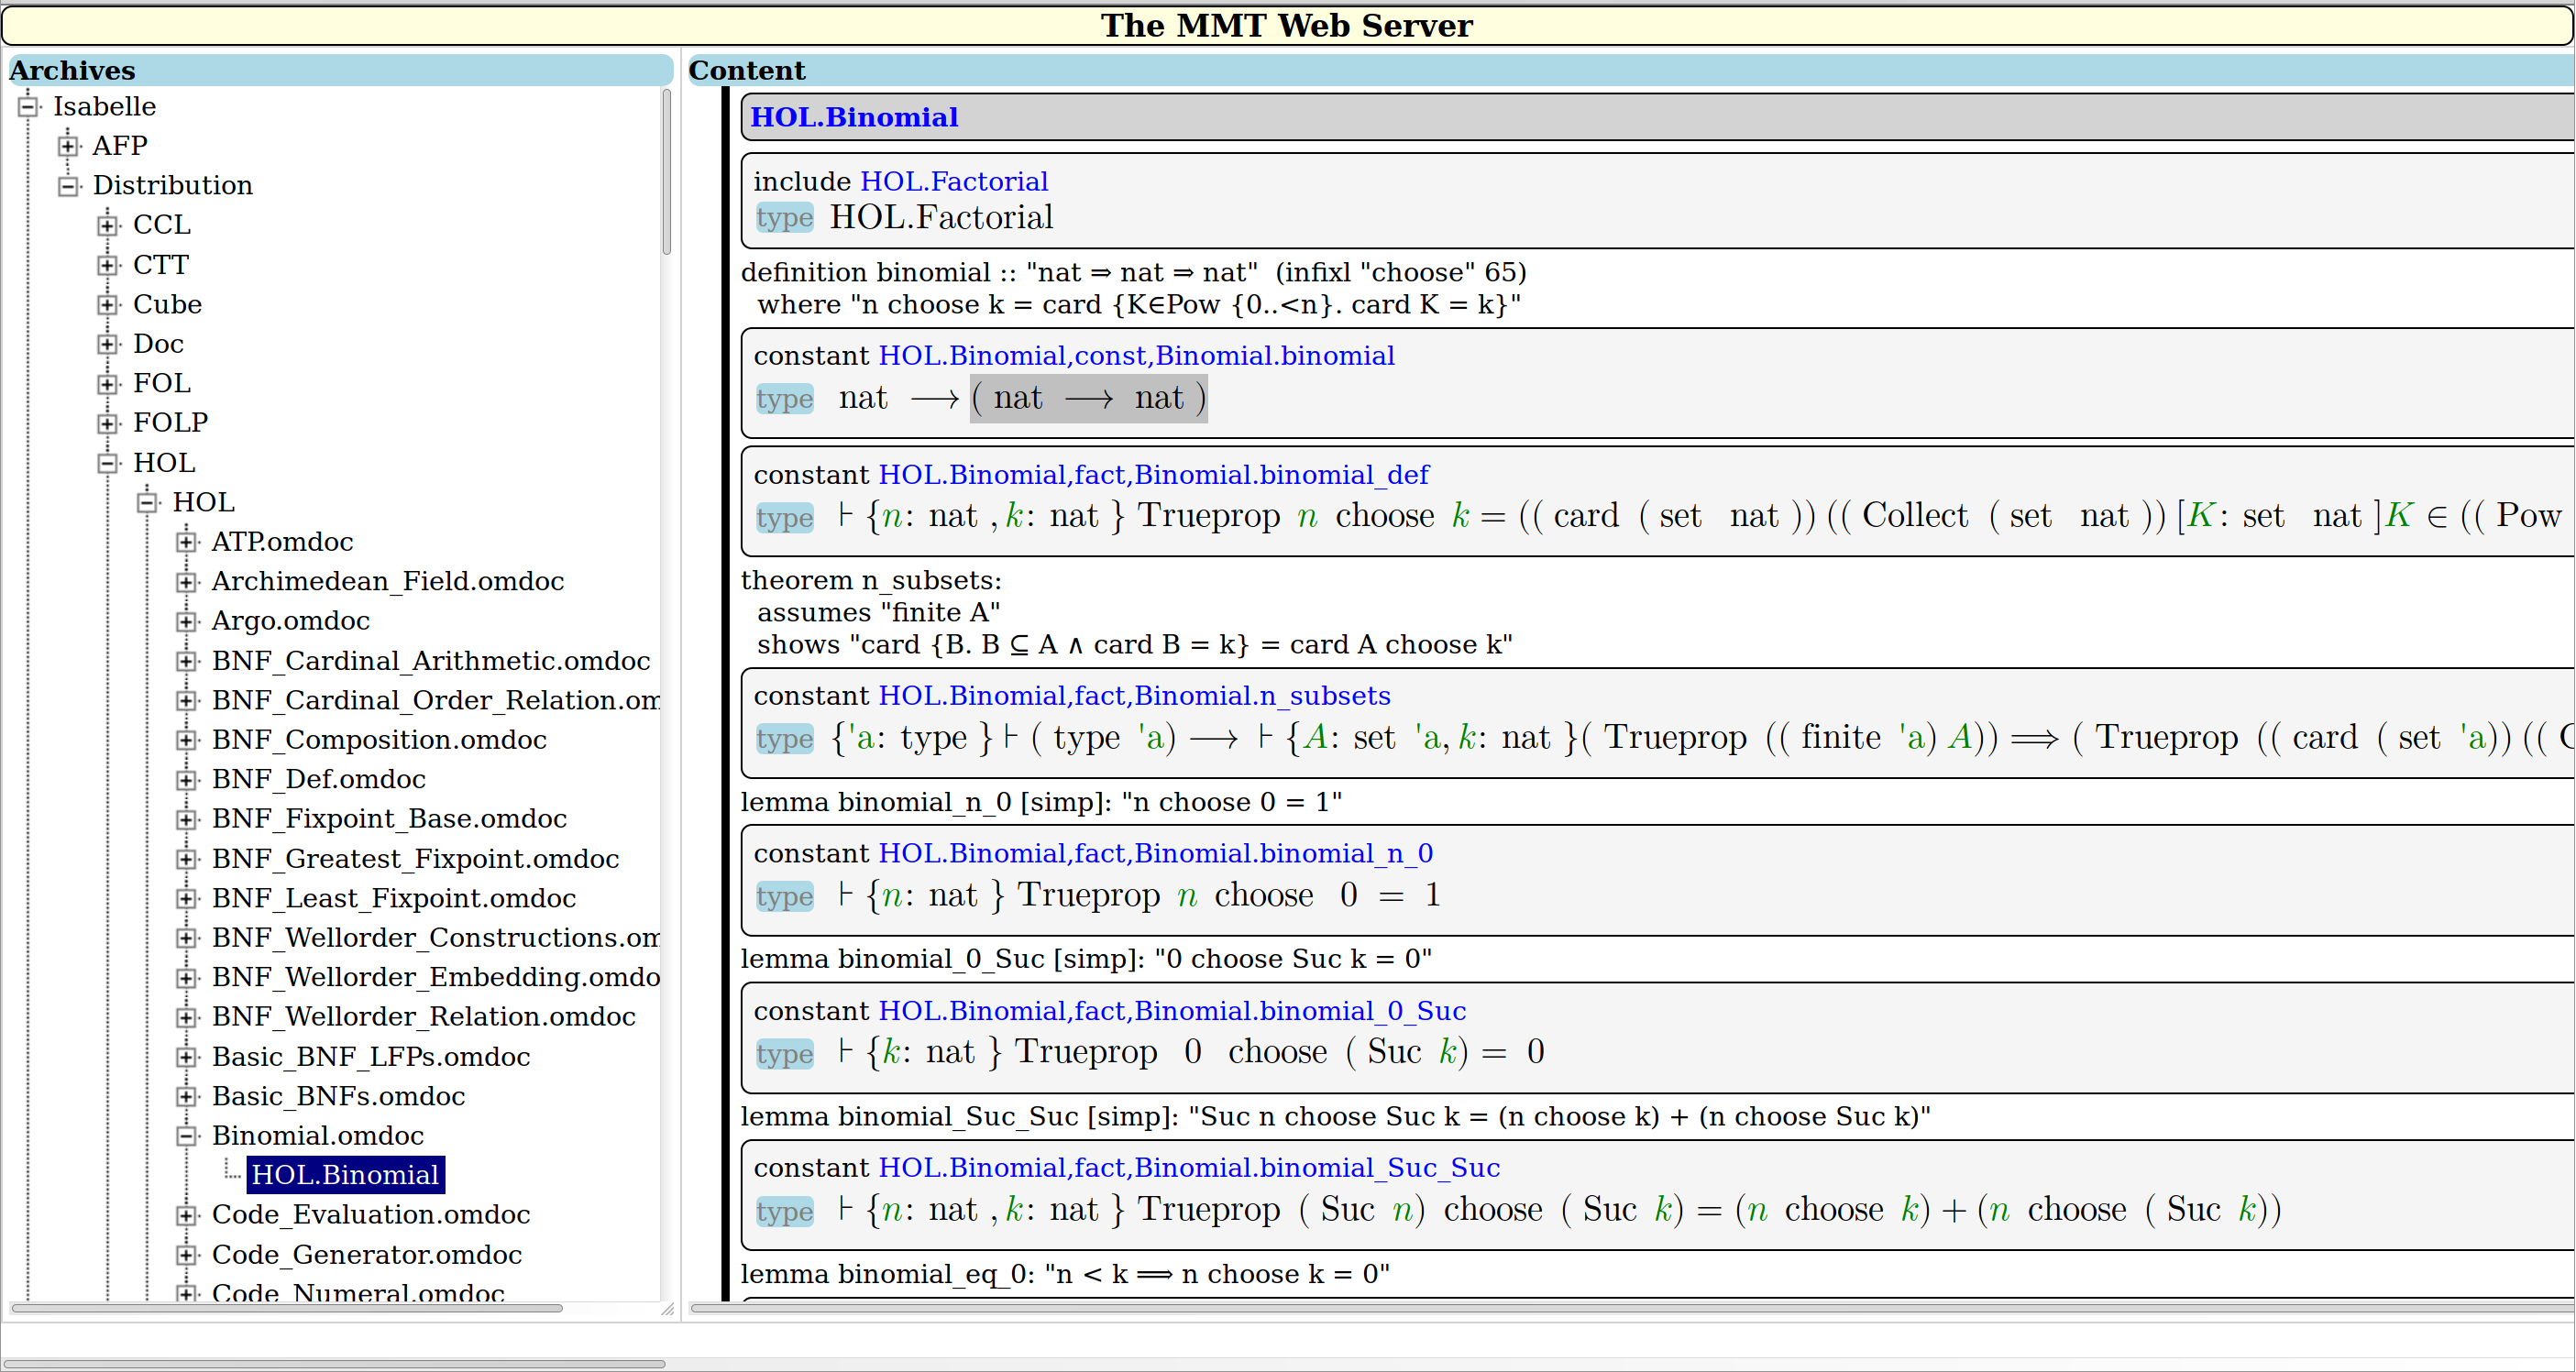
\includegraphics[width=\textwidth]{isabelle_mmt}
  \caption{MMT browser showing Isabelle content}\label{fig:isabellemmt}
\end{figure}

\paragraph{Module System}
All module system--level Isabelle entities are represented as MMT theories and morphisms.
These use a manually written MMT meta-theory that formalizes Isabelle/Pure --- the logic underlying Isabelle.

Besides plain Isabelle theories, this includes the order-sorted algebra of \emph{type classes} (subclass relation) and \emph{type arities} (image behavior of type constructors wrt.\ type class domains and ranges) in the sense of Nipkow and Prehofer \cite{Nipkow-Prehofer:1993} as well as locales in the sense of Ballarin \cite{Ballarin2014} and type classes as special locale interpretations in the sense of Haftmann and Wenzel \cite{Haftmann-Wenzel:2006:classes,Haftmann-Wenzel:2009}.

  Isabelle locales are \emph{named contexts} with type parameters
  (implicit), term parameters (\textbf{fixes}), and premises
  (\textbf{assumes}). Within such a ``little theory'' it is possible
  to spell out definitions, statements, proofs as usual --- all
  results are understood as relative to the context. The foundations
  will contain an extra prefix of type variables, term abstractions
  and assumptions according to the context.

  The export of locales preserves some of its internal structure,
  notably the locale dependency relation stemming from the
  construction of locales and sub-locales (by definition), as well as
  later locale interpretations (by proof).

  Type classes are special locales with a single type parameter and a
  canonical locale interpretation to connect \emph{type class
    parameters} (polymorphic constants with class constraints) to
  \emph{locale parameters} (fixed variables of the context). The
  export shows the result of the interpretation, but \emph{without} an
  explicit report on their connection.


\paragraph{Declarations}
Every declaration in a theory-like scope is represented as an MMT declaration.
This includes \textbf{types} (base types and type constructors),
  term \textbf{constants} (including functions, binders, quantifiers
  as higher-order constants), \textbf{axioms} (including equational
  axioms that count as primitive definitions), and \textbf{theorems}
  (propositions with a proof).

Isabelle definitions become equational axioms in MMT.
This includes theorems, which are treated as defined constants in MMT via the Curry-Howard representation.
However, the actual proofs, which become the definientia of these constants, are not exported by default (proof terms are prohibitively large), but it is possible to reconstruct the source text in the Isabelle/Isar proof language from the position information.

Type definitions in the sense of Gordon and
  Pitts \cite{pitts93} are interpreted
  definitionally within the standard semantics of the HOL
  logic. The export facility provides access to the key
  information: the old representing type, the new abstract type, the
  name of the morphisms between the two with the axiom stating the
  relation.
  This information allows recovering HOL typedefs faithfully, where
  Isabelle/Pure theory content would only show the individual
  particles. It also serves as an example to ``query'' derived
  specification mechanisms in Isabelle/ML, to expose its own level of
  abstraction to the exporter.
  
Term constants with indication of derived specifications
  mechanisms, e.g.\ \textbf{primrec} functions, \textbf{inductive} or
  \textbf{coinductive} relations are handled by querying generic
  information in Isabelle/Pure about functional or relation
  specifications (so-called ``Spec Rules''). The Isabelle/HOL
  implementations provide this data on their own account.

\paragraph{Expressions}
The expressions of Isabelle's $\lambda$-calculus are represented as MMT terms.
This part of the translation is relatively straightforward and similar to previous exports to OMDoc/MMT (e.g., \cite{KalRab:hollight:14,KohMueOwr:mpagsiuf17,MueRabSac:cltg19}).
Only the treatment of variables warrants further description, and we focus on it in the sequel.

Isabelle variables come in various flavours: free variables (e.g.\
\verb,x,), schematic variables with index (e.g. \verb,?x10,) and bound
variables (e.g. \verb,x, in $\lambda$\verb,x::,$\tau$\verb,. x, which
is concrete syntax for the de-Bruijn index abstraction
\verb;Abs (x, ;$\tau$\verb;, B.0); where \verb,x, is retained as a
comment). To fit smoothly into the lambda-calculus of MMT, variable
names are standardized as follows:

Schematic variables are renamed to fresh free variables. Since
  schematic variables are morally like a universal quantifier prefix,
  this preserves the logical meaning of a formala (e.g.\ a theorem
  statement).

Bound variable comments in abstractions are renamed locally to
  avoid clashes with free variables in the same scope. Thus the
  comment can be used literally in MMT/LF as named abstraction,
  ignoring the unnamed de-Bruijn index representation of Isabelle.

Finally, Isabelle type variables are decorated with type class constraints,
e.g.\ \verb,'a::order, for types that belong to the class \verb,order,
defined in the Isabelle/HOL library (e.g.\ \verb,nat, with its
standard order): this ensures certain \emph{operations} with a link to
overloaded term constants (e.g.\ \verb,less :: 'a => 'a => bool,), as
well as logical \emph{premises} on these operations (e.g.\ stating
that \verb,less, is a strict order on the type).

Isabelle class operations are managed by extra-logical means, e.g.\ by
the code-generator for Haskell or Standard ML, to produce the expected
\emph{dictionary construction} to eliminate the implicit
overloading. In MMT this will merely result in uncontrolled
polymorphism: constant definitions consist of multiple
(non-overlapping) equational specifications depending on the type
argument.

Isabelle class premises become logical constraints in a
straight-forward manner: a type class is a predicate over types in LF,
so \verb,'a::c, means that the predicate \verb,c, applied to type
\verb,'a, holds. Statements with class constraints
$\phi($\verb,'a::c,$)$ are augmented by a prefix of preconditions
\verb,'a::c,${} \Longrightarrow \phi($\verb,'a,$)$, effectively
eliminating the constraint within the logic.

\paragraph{Identifiers}
Isabelle constants live in separate name spaces (for types, terms,
theorems etc.).  For example, there could be a type \verb,Nat.nat, and
a term constant of the same name (e.g.\ an operation to make a natural
number). Qualification is usually by the theory \emph{base} name, not
the session-qualified long name; in rare situations, there is no
theory qualification at all. In order to have all entities coexist
within one big space of individuals in MMT, we use a triple that
consists of (\emph{long-theory-name}, \emph{entity-name},
\emph{entity-kind}) written as URI like as follows:

\begin{quote}
\texttt{https://isabelle.in.tum.de?}\emph{long-theory-name}\texttt{?}\emph{entity-name}\texttt{|}\emph{entity-kind}
\end{quote}

\noindent For example, \texttt{https://isabelle.in.tum.de?HOL.Nat?Nat.nat|type} refers to the type of natural numbers in the Isabelle/HOL library.


% % % % % % % % % % % % % % % % % % % % % % % % % % % % % % % % % % % % % % % % % % % % % % % % % % %
\subsubsection{Exporting Relational Knowledge in ULO Format}

Relations between formal items are output as RDF/XML triples,
  bypassing MMT and its OMDoc format; see also
  \cite[\S3.1]{ConKohMue:rdaml19}.  This also captures some aspects of
  inductive and primitive recursive definitions via
  \verb,ulo:inductive-on,. In addition to that paper, there is now
  full coverage of theorem dependencies via \verb,ulo:uses,, spanning
  a rather large dependency graph over the source text: it relates
  theorem statements with used constants and proofs with used
  theorems.  



\paragraph{Individuals}
Formal entities are identified by their \emph{name} and \emph{kind} as follows:
\begin{compactitem}
\item The name is a long identifier (with dot as separator, e.g.\ \texttt{Nat.Suc}) that is unique within the current theory context (including the union of all theory imports). Long names are managed by namespaces within the formal context to allow partially qualified names in user input and output (e.g.\ \texttt{Suc}). The structure of namespaces is known to the prover, and not exported.
\item The kind is a short identifier to distinguish the namespaces of formal entities, e.g.\ \texttt{type} for type constructors, \texttt{const} for term constants, \texttt{fact} for lists of theorems that are recorded in the context, but also non-logical items like \texttt{method} (Isar proof methods), \texttt{attribute} (Isar hint language) etc.
\end{compactitem}

\noindent
This name/kind scheme is in contrast to usual practice in universal $\lambda$-calculus representations like MMT/LF, e.g.\ there could be a type \texttt{Nat.nat} and a separate term constant of the same name.  Moreover the qualification in long names only uses theory base names, not their session-qualified long name (which was newly introduced in Isabelle2017). So in order to support one big space of individuals over all Isabelle sessions and theories, we use the URI format that was already used for identifiers above.

\paragraph{Logic}
The primitive logical entities of Isabelle/Pure are types, terms, and theorems (facts).
Additionally, Isabelle supports various theory-like structures.
These correspond our declaration classes as follows:
\begin{compactitem}
\item \ind{theory} refers to global \textbf{theory} and local \textbf{locale} contexts. There are various derivatives of \textbf{locale} that are not specifically classified, notably \textbf{class} (type classes) and \textbf{experiment} (locales with inaccessible namespace).
\item \ind{type} refers to \emph{type constructors} of Isabelle/Pure, and object-logic types of many-sorted FOL or simply-typed HOL. These types are syntactic, and not to be confused with the ``propositions-as-types'' approach in systems like Coq. Dependent types are represented as terms in Isabelle.
\item \ind{function} refers to \emph{term constants}, which are ubiquitous in object-logics and applications. This covers a broad range of formal concepts, e.g.\ logical connectives, quantifiers (as operators on suitable $\lambda$-terms), genuine constants or mathematical functions, but also recursion schemes, or summation, limit, integration operators as higher-order functions.
\item \ind{statement} refers to individual theorems, which are projections from the simultaneous \texttt{fact} lists of Isabelle.  Only the head statement of a theorem is considered, its proof body remains abstract (as reference Isar to proof text).
Theorems that emerge axiomatically (command \textbf{axiomatization}) are marked as \ind{primitive}, properly proven theorems as \ind{derived}, and theorems with unfinished proofs (command \textbf{sorry}) as \ind{experimental}.
\end{compactitem}

\noindent The \ind{specifies} and \ind{specified-in} relations connect theories and locales with their declared individuals.
The \ind{uses} relation between those represents syntactic occurrence of individuals in the type (or defining term) of formal entities in Isabelle: it spans a large acyclic graph of dependencies. Again, this excludes proofs: in principle there could be a record of individuals used in the proof text or by the inference engine, but this is presently unimplemented.

The \ind{source-ref} property refers to the defining position of formal entities in the source.
Thanks to Isabelle/PIDE, this information is always available and accurate: the Prover IDE uses it for highlighting and hyperlinks in the editor view. Here we use existing URI notation of MMT, e.g.\ \url{https://isabelle.in.tum.de/source/FOL/FOL/FOL.theory#375.19.2:383.19.10} with offset~/ line~/ column of the two end-points of a text interval.

The \ind{check-time} and \ind{external-size} properties provide some measures of big theories in time (elapsed) and space (sources).  This is also available for individual commands, but it is hard to relate to resulting formal entities: a single command may produce multiple types, consts, and facts simultaneously.

\paragraph{Semi-formal Documents}
We use \ind{section} for the six levels of headings in Isabelle documents: \textbf{chapter}, \textbf{section}, \dots, \textbf{subparagraph}.  These are turned into dummy individuals (which are counted consecutively for each theory).

\ind{file}, \ind{folder}, \ind{library} are presently unused.
They could refer to the overall project structure Isabelle document sources in the sense of~\cite{Wenzel:IIdsflitd18}, namely as \emph{theories} (text files), \emph{sessions} (managed collections of theories), and \emph{project directories} (repository with multiple session roots).

For document metadata, we use the Dublin Core ontology.  The Isabelle command language has been changed to support a new variant of \emph{formal comment}. With one keystroke, the presentation context of a command may be augmented by arbitrary user-defined marker expressions. Isabelle/Pure already provides \texttt{title}, \texttt{creator}, \texttt{contributor} etc.\ from \S\ref{sec:objprops}: they produce PIDE document markup that Isabelle/MMT can access and output as corresponding RDF.

This approach allows to annotate theory content \emph{manually}: a few theories of \texttt{HOL-Algebra} already use the new feature sporadically. For automatic marking, metadata of AFP entries is re-used for their theories. One could also digest comments in theory files about authors, but this is presently unimplemented.


\subsubsection{Statistics}\label{sec:stats}

We present some statistics\footnote{Versions: Isabelle/9c60fcfdf495, AFP/d50417d0ae64, MMT/e6fa4b852bf9.}.
This gives an idea about overall size and scalability of the export facilities so far.
The datasets are publicly available from \url{https://gl.mathhub.info/Isabelle}.

{\tiny
\begin{center}
\begin{tabular}{cl||r|r||r|r|r|r|r||r|r}
  & Library                       & Individuals & Relations  & Theories & Locales  & Types      & Constants & Statements  & RDF/XML    & elapsed \\
  &                               &             &            &          &          &            &           &             & file size  & time \\\hline
  \isabelle & Distribution        &     103,873 &  2,310,704 &      535 &     496  &   235      & 8,973     &     88,960  & 188\,MB    & 0.5h \\
            & only group                                                                                                    
                    \texttt{main} &             &            &          &          &            &           &             &            & \\\hline
  \isabelle & Distribution+AFP    &   1,619,889 & 36,976,562 &    6,185 &  4,599   & 10,592     & 215,878   &  1,359,297  & 3,154\,MB  & 16.5h \\
            & without \verb,very_slow,
                                  &             &            &          &          &            &           &             &            & \\\hline
%  \coq      & All 49 Libraries    & 383,527     & 11,516,180 &    1,979 & -        &  6,061     & -         &  161,736    & 452\,MB    & \\
\end{tabular}
\end{center}}

%%% Local Variables:
%%% mode: latex
%%% mode: visual-line
%%% fill-column: 5000
%%% TeX-master: "report"
%%% End:

%  LocalWords:  subsubsection texttt texttt paulson700 emph Wenzel:IIdsflitd18 organized verb,export_theory verb,export_proofs externalize verb,isabelle verb,isabelle consts fig:isabellemmt includegraphics textwidth isabelle_mmt arities wrt Prehofer Nipkow-Prehofer:1993 Ballarin Ballarin2014 textbf pitts93 primrec coinductive ednote pvs verb,x verb,order verb,nat verb,less verb,c Longrightarrow noindent ConKohMue:rdaml19 verb,ulo:inductive-on verb,ulo:uses compactitem axiomatization sec:objprops hline verb,very_slow


\subsection{Applications}\label{sec:uloappl}
% \ednote{FR: Picking 1 of the 3 queries given here is enough as an example.
% The paragraph 'Additional Examples' should be removed, and 1-2 of the difficult queries given there should be given as advanced examples.
% Try to give one screenshot of the result of a complex query. Say how many results the queries return.}

In this section, we evaluate the ULO framework, i.e. the ULO ontology and the generated RDF data by showing how they could be exploited using standard tools of the Semantic Web tool stack.

We have set up an instance of Virtuoso Open-Source Edition\footnote{\url{https://github.com/openlink/virtuoso-opensource}}, which reads the exports described in Section~\ref{sec:isabelle-export} and provides a web interface with a SPARQL endpoint to experiment with the ULO dataset.
Then we have tried several queries with promising results (just one shown below for lack of space).
The queries are not meant to be a scientific contribution per se: they just show how much can be accomplished with the ULO dataset with standard tools in one afternoon.

\paragraph{Example query: all recursive functions on $\mathbb{N}$} For this, we use the \lstinline|ulo:inductive-on| relation to determine inductive definitions on a type \lstinline|?y|, which we restrict to one that is aligned with the type \lstinline|nat_lit| of natural numbers from the interface theory \lstinline|NatLiterals| in the Math-in-the-Middle Ontology.
\begin{lstlisting}
SELECT ?x ?y WHERE {
  ?x ulo:inductive-on ?y .
  http://mathhub.info/MitM/Foundation?NatLiterals?nat_lit ulo:aligned-with ?y . }
\end{lstlisting}
Note that we use alignments~\cite{MueGauKal:cacfms17} with concepts from an interface theory as a way of specifying ``the natural numbers'' across theorem prover libraries. The result is a list of pairs: each pair combines a specific implementation of natural numbers (Isabelle has several, depending on the object-logic), together with a function defined by reduction on it. A subset of the results of this query are shown in Figure~\ref{fig:query}.

\begin{figure}[t]\centering
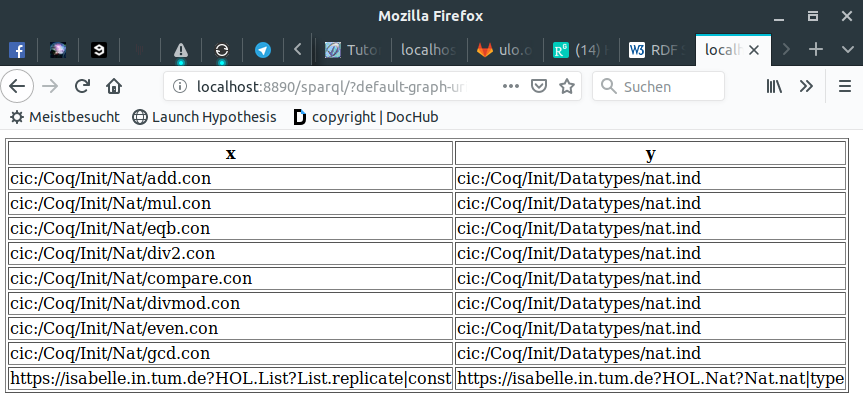
\includegraphics[width=\textwidth]{ulo_queryresult}
\caption{Virtuoso Output for the Example Query using Alignments}\label{fig:query}
\end{figure}

\ednote{check if Dennis can supply Isabelle screenshots}

%Similarly,  we can e.g. use the \lstinline|ulo:orcid| and \lstinline|dcterms:creator| properties to e.g. query for all theorems by Michael Kohlhase or Claudio Sacerdoti Coen using their ORCID.

\paragraph{Transitive Queries} The result of the query above only depends on the explicitly generated RDF triples. Semantic Web tools that understand OWL allow more complex queries. % For example, if we want to query for \emph{all theorems whose proofs depend on statements with incomplete proofs}, it is sufficient to specify in the ontology that \ind{uses} is transitive, and add a property to identify incomplete proofs.
For example, Virtuoso implements custom extensions that allow for querying the transitive closure of a relation. The resulting query syntax is a little convoluted, and we omit some details in the example below.
\begin{lstlisting}
SELECT ?o ?dist WHERE { {
      SELECT ?s ?o WHERE { ?s ulo:declares ?o }
    }
    OPTION ( TRANSITIVE, t_distinct, t_in(?s), t_out(?o), t_min (1),
             t_max (10), t_step ('step_no') as ?dist ) .
    FILTER ( ?s = <https://isabelle.in.tum.de?HOL.Nat> )
  }
ORDER BY ?dist DESC 2
\end{lstlisting}
The above code queries for all symbols recursively declared in the (effectively randomly chosen) Theory \texttt{HOL.Nat} declaring the natural numbers and associated concepts; the output for that query is shown in Figure \ref{fig:query2}.


\begin{figure}[ht]\centering
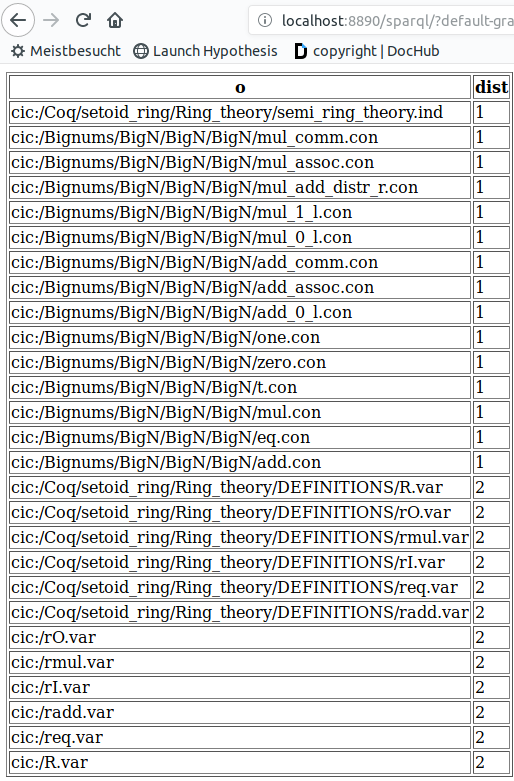
\includegraphics[width=0.5\textwidth]{ulo_queryresult2}
\caption{Virtuoso Output for the Transitive Example Query}\label{fig:query2}
\end{figure}

%then we have to use that the \ind{ulo:uses} is transitive.
%This is specified in the OLW2 implementation ULO ontology and can be used by sufficiently powerful tools (e.g. Virtuoso).
%Given that Virtuoso implicitly computes the transtive closure we can answer the query using a very similar query as the one above (given an alignment for proof gap objects).

Interesting examples of library management queries which can be modeled in SPARQL (and its various extensions, e.g. by rules) are found in~\cite{conf/lpar/AspinallDL12}. Instead~\cite{AGSTZ:ContMathSearchWhelp04,MKM04:AspertiS04} show examples of interesting queries (approximate search of formulae up to instantiation or generalization) that can be implemented over RDF triples, but that requires an extension of SPARQL with subset and superset predicates over sets.
% \ednote{DM: Add detailed examples (transitivity?)}
%\begin{center}
%\begin{tabular}{|c|c|}\hline
%	\lstinline|x| & \lstinline|y| \\\hline\hline
%	\tiny\lstinline>https://isabelle.in.tum.de?HOL.List?List.replicate|const> & \tiny\lstinline>https://isabelle.in.tum.de?HOL.Nat?Nat.nat|type> \\\hline
%	\tiny\lstinline|cic:/Coq/Init/Nat/add.con| & \tiny\lstinline|cic:/Coq/Init/Datatypes/nat.ind| \\\hline
%	\tiny\lstinline|cic:/Coq/Init/Nat/mul.con| & \tiny\lstinline|cic:/Coq/Init/Datatypes/nat.ind| \\\hline
%	\tiny\lstinline|cic:/Coq/Init/Nat/div2.con| & \tiny\lstinline|cic:/Coq/Init/Datatypes/nat.ind| \\\hline
%\end{tabular}
%\end{center}
%
%\paragraph{All theorems by Michael Kohlhase or Claudio Sacerdoti Coen}\ 
%\begin{lstlisting}
%SELECT ?x WHERE {
% ?x [ulo:theorem ?y ; dcterms:creator ?z]
% {?z ulo:orcid "0000-0002-4360-6016"} 
%   UNION
% {?z ulo:orcid "0000-0002-9859-6337"} }
%\end{lstlisting}
%
%\paragraph{All theorems with incomplete Proofs}\
%\begin{lstlisting}
%SELECT ?x WHERE {
%  ?x [ulo:proof ?y ; ulo:uses ?z]
%  ?z ulo:aligned-with http://mathhub.info/MitM?proofs?gap
%  OPTION ( TRANSITIVE, t_distinct, t_in(?x),t_out(?z)) }
%\end{lstlisting}
%This query is similar to the one about all inductive functions above, only that we use transitivity for the \lstinline|ulo:uses| relation (SPARQL syntax simplified).\ednote{MK: I have copied this by pattern matching from \url{https://virtuoso.openlinksw.com/tutorials/sparql/SPARQL_Tutorials_Part_5/SPARQL_Tutorials_Part_5.html} without understanding much.\\DM: Doing this properly gets ugly and elaborate; I would leave it simplified.}
%
%\paragraph{Additional examples} include
%\begin{itemize}
%\item Authors with the slowest proofs (in verification)
%\item Libraries ordered by dependency and check-time
%\item Dependency paths by cumulative check time
%\item Subgraphs by Topology; e.g. all situations of the form
%  \begin{tikzpicture}[baseline=(c.base),xscale=1.4,yscale=.8]
%    \node (lo) at (0,1) {$\bullet$};
%    \node (ro) at (1,1) {$\bullet$};
%    \node (lu) at (0,0) {$\bullet$};
%    \node (ru) at (1,0) {$\bullet$};
%    \node (c) at (.5,.5){};
%    \draw[include] (lu) -- (lo) ;
%    \draw[include] (ru) -- (ro);
%    \draw[struct] (lo) -- node[above]{\tiny deps} (ro);
%  \end{tikzpicture}
%  in a given library.
%\end{itemize}
%%% Local Variables:
%%% mode: latex
%%% mode: visual-line
%%% fill-column: 5000
%%% TeX-master: "report"
%%% End:

%  LocalWords:  ednote mathbb MueGauKal:cacfms17 centering includegraphics textwidth queryresult emph hline texttt BigNring AGSTZ:ContMathSearchWhelp04,MKM04:AspertiS04 generalization


%%% Local Variables:
%%% mode: latex
%%% mode: visual-line
%%% fill-column: 5000
%%% TeX-master: "report"
%%% End:

%  LocalWords:  ednote sec:uloappl mathbb Makarius optimized sec:appl ulo_appl
